
\chapter{Scalars}
\minitoc 

\noindent
\begin{minipage}{0.5\textwidth}
Scalar values can be associated to each vertex. Scalar values
can be displayed when scalar display mode is active. To
activate/deactivate scalar display mode, click on ``
\includegraphics[scale=0.7]{images/pixmap/show_color_scale.png}".
When active, the rainbow colour scale (see Fig. \ref{rainbow_colour_scale}) shows up in the
bottom-right part of the 3D rendering window.
\end{minipage}    
\begin{minipage}{0.5\textwidth}\centering
  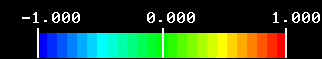
\includegraphics[scale=0.5]{images/Scalars_renreding/Colour scale.png}
 \captionof{figure}{Rainbow colour scale, showing a
``min" range display value of -1, a
``max" range display value of 1, and a
middle range display value of 0.
}
\label{rainbow_colour_scale}
 \end{minipage} 
\noindent


\section{Show scalar rendering options window.}
\noindent
\begin{minipage}{0.5\textwidth}
Displayed scalars and scalar associated
colour scales can aslo be onpened by
clicking on ``
\includegraphics[scale=0.7]{images/pixmap/edit_color_scale.png}" (see Fig. \ref{Scalar_rendering_options_window}).\\
\noindent
\textbf{\underline{Available controls:}}\\
\textit{Chose active scalar}: please chose among
the available scalars (see below for further
information).\\
\textit{Chose colour scale}: please chose among
the available colour scales (see below for
further information).
\end{minipage}    
\begin{minipage}{0.5\textwidth}\centering
  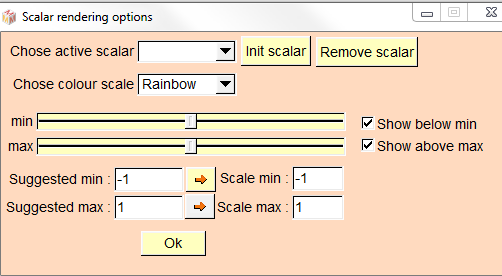
\includegraphics[scale=0.5]{images/Scalars_renreding/Colour_scale_rendering_window.png}
\captionof{figure}{Scalar rendering options window}	
\label{Scalar_rendering_options_window}
 \end{minipage} 
\noindent
\textit{Init scalar}: set current active scalar values to ``0" for all selected objects.
Remove scalar : removes active scalar for all selected objects. This option is useful if you plan to save surfaces in the .vtk format and do not want ISE-MeshTools to save associated scalar values (this will save some disk space).\\
\textit{min}: changes the minimal value of the active colour scale.\\
\textit{max}: changes the maximal value of the active colour scale.\\
\textit{Show below min}: if active, all vertices with an associated active scalar value below ``min" will be drawn using the colour situated at the leftmost part of the active colour scale. If not, these vertices will be transparent.\\
\textit{Show below max}: if active, all vertices with an associated active scalar value above ``max" will be drawn using the colour situated at the rightmost part of the active colour scale.\\
\textit{Suggested min}: suggested ``min" range display value. This value is computed in order to use the
colour scale at its best.\\
\textit{Suggested max}: suggested ``max" range display value. This value is computed in order to use the
colour scale at its best.\\
``
\includegraphics[scale=0.7]{images/pixmap/s_right_132.png}": Set min/max to suggested min/max, respectively.\\
\textit{Scale min}: current ``min" range display value.\\
\textit{Scale max}: current ``max" range display value.
\textit{Ok}: applies changes.


\section{Scalars: distance from camera (Depth).}
\noindent
\begin{minipage}{0.5\textwidth}
Computes distance from camera for all vertices of
all selected objects. This option may offer a better
perception of the 3D structure of an object on a
2D screen representation.
\end{minipage}    
\begin{minipage}{0.5\textwidth}\centering
  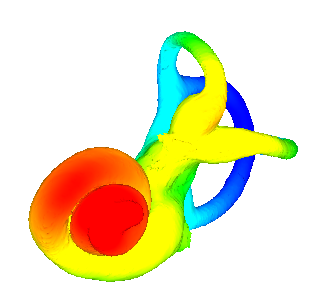
\includegraphics[scale=0.5]{images/Scalars_renreding/Depth.png}
 \captionof{figure}{Example of 3D rendering of ``Depth" scalars.
Scalar mode is active, the rainbow colour scale
is used.
}
\label{depth_scalar}
 \end{minipage} 
\noindent



\section{Scalars : compute vertice curvature.}
\section{Scalars: distance from camera (Depth).}
\noindent
\begin{minipage}{0.5\textwidth}
vtkCurvatures filter is implied in this option.\\
vtkCurvatures filter offers 4 ways to compute surface's
curvature at each vertex (see Fig. \ref{curvatures}):\\
- Principal maximal curvature\\
- Principal minimal curvature\\
- Gaussian curvature\\
- Mean curvature.\\
See vtkCurvatures' documentation for further details.

\end{minipage}    
\begin{minipage}{0.5\textwidth}\centering
  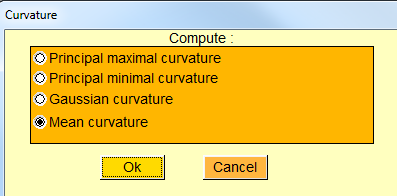
\includegraphics[scale=0.5]{images/Scalars_renreding/Curvature_window.png}
 \captionof{figure}{Curvature window}
\label{curvature_window}
 \end{minipage} 
\noindent

\begin{figure}
  \centering
  \includegraphics[scale=0.3]{images/Scalars_renreding/Curvatures.pdf} 
	\caption{
Examples of 3D rendering of ``Curvature" scalars. Scalar mode is active, the rainbow colour scale is used. Specimen : enamel dentine junction (EDJ) of the second superior molar of a juvenile medieval human from Sains-en-Gohelle (France). Specimen number : SP07. Image credit: Mona Le Luyer (PACEA, Bordeaux).}
\label{curvatures}
 
\end{figure}

\section{Scalars: compute thickness.}
\noindent
\begin{minipage}{0.5\textwidth}
Thickness within an object (see Fig. \ref{thickness}) is defined the following way: for a
given vertex, the minimal distance between this vertex and other
vertices in the direction opposite to that of the surface's normal
is computed. In order to minimize computation time, a maximal
distance (Maximal thickness (mm) ) is asked to the user, in order
to reduce the amount of vertices investigated at a given location.
\end{minipage}    
\begin{minipage}{0.5\textwidth}\centering
  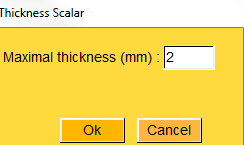
\includegraphics[scale=0.5]{images/Scalars_renreding/Thickness_window.png}
 \captionof{figure}{Thickness scalar window}
\label{thickness_window}
 \end{minipage} 
\noindent





\section{Scalars: compute thickness between two objects.}
\noindent
\begin{minipage}{0.5\textwidth}
Thickness between tow objects is defined the following way (see Fig. \ref{thickness2}):
for a given vertex of the impacted object, the minimal distance
between this vertex and other vertices of the observed surface in
the direction opposite to that of the impacted surface's normal
is computed. Again, in order to minimize computation time, a
maximal distance (Maximal thickness (mm) ) is asked to the user,
in order to reduce the amount of vertices investigated at a given
location. Only selected surfaces appear in the impacted object
and observed object lists.
\end{minipage}    
\begin{minipage}{0.5\textwidth}\centering
  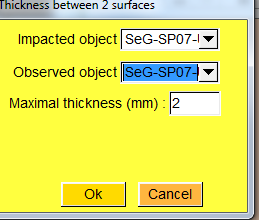
\includegraphics[scale=0.5]{images/Scalars_renreding/Thickness_window2.png}
 \captionof{figure}{Thickness between 2 surfaces window}
\label{thickness_window2}
 \end{minipage} 
\noindent


\noindent
\begin{minipage}{0.5\textwidth}\centering
 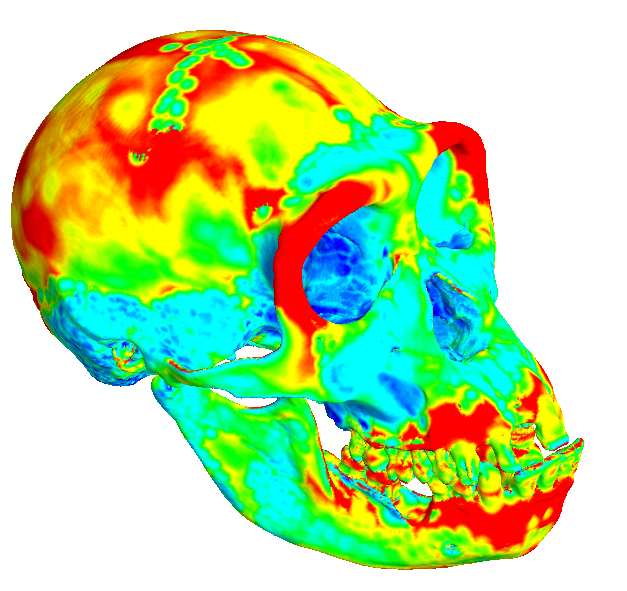
\includegraphics[scale=0.3]{images/Scalars_renreding/Thickness2.png}
 \captionof{figure}{Example of 3D rendering of ``Thickness" of the
3D model ot the type specimen of \textit{Pan paniscus}
(downloadable on \href{http://www.metafro.be/primates/panpaniscustype}{Metafro.be}). Scalar mode is active,
the rainbow colour scale is used.
Thickness between 2 surfaces
window}
\label{thickness}

\end{minipage}    
\begin{minipage}{0.5\textwidth}\centering
  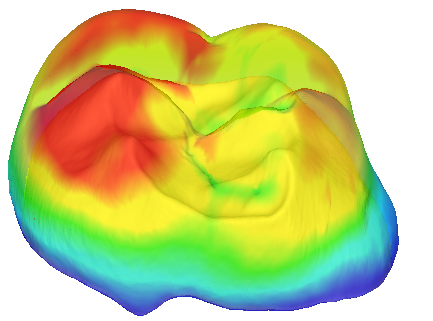
\includegraphics[scale=0.5]{images/Scalars_renreding/thickness_.png}
 \captionof{figure}{Example of 3D rendering of ``Thickness" between
two objects' scalars. Scalar mode is active,
the rainbow colour scale is used. Impacted
object : enamel surface of SP07 specimen (see
above for details). Observed object : enameldentine
junction's surface (EDJ) of SP07 specimen.}
\label{thickness2}
 \end{minipage} 
\noindent





\section{Smooth active scalars (Gaussian blur).}
Active scalars are ``smoothed" the following way : for each vertex, a new scalar value is computed as
the mean of the scalar values of all neighbouring vertices (see Fig. \ref{smoothing_scalars}).
\begin{figure}
  \centering
  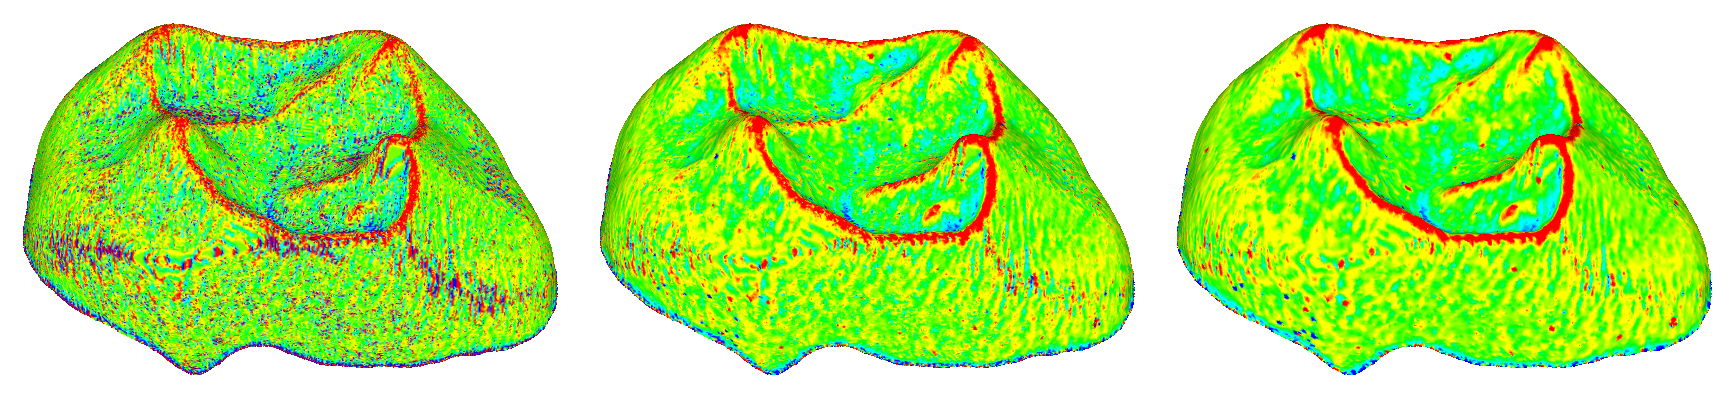
\includegraphics[scale=0.25]{images/Scalars_renreding/Smooth_012.png} 
	\caption{Smoothing scalars. Examples of 3D rendering of ``Mean Curvature" scalars. Scalar mode is active, the rainbow colour scale is used. Left : ``raw" mean curvature. Middle : mean curvature scalars smoothed once. Right : mean curvature scalars smoothed twice. Specimen: EDJ of SP07 specimen.}
\label{smoothing_scalars}
 
\end{figure}




\section{Saving and loading scalars.}
Computed scalars can be saved inside the .vtk surface files. In order to access scalar values into other
software (such as a text editor), save the .vtk files in ASCII format. Saved scalars can be reloaded into
ISE-MeshTools. Saving surfaces into .vtk format provides an efficient means to store and exchange
computed scalars.
